\documentclass[tikz,border=6pt]{standalone}

% общий стиль (подключается через TEXINPUTS)
% tikz-style.tex (общий стиль для всех TikZ-картинок)
\RequirePackage[T1,T2A]{fontenc}
\RequirePackage[utf8]{inputenc}

% Palatino-подобный шрифт (как в MathJax часто воспринимается «более вытянутым»)
\RequirePackage{txfonts}
% txfonts даёт предупреждение по кириллице (T2A/txr не определён).
% Оставляем txfonts для математики, а текстовый шрифт возвращаем на Computer Modern,
% чтобы не искать T2A/txr и убрать предупреждения.
\renewcommand{\rmdefault}{cmr}
\renewcommand{\sfdefault}{cmss}
\renewcommand{\ttdefault}{cmtt}

\RequirePackage{tikz}
\RequirePackage{xcolor}
\usetikzlibrary{calc}

% цвета
\definecolor{lightgreen}{RGB}{214,234,214}
\definecolor{darkgreen}{HTML}{0B7A0B}
\definecolor{darkred}{HTML}{DF0000}

\definecolor{midgreen}{HTML}{2E9B2E}
\definecolor{palegreen}{RGB}{235,246,235}
\definecolor{olivegreen}{HTML}{3E6B2F}

\definecolor{lightred}{RGB}{255,220,220}
\definecolor{midred}{HTML}{E04545}
\definecolor{darkred2}{HTML}{A80000}

\definecolor{lightblue}{RGB}{220,232,255}
\definecolor{midblue}{HTML}{2E5BD6}
\definecolor{darkblue}{HTML}{0B2E8A}

\definecolor{lightgray}{RGB}{240,240,240}
\definecolor{midgray}{RGB}{170,170,170}
\definecolor{darkgray}{RGB}{80,80,80}

\definecolor{vtxfill}{RGB}{86,193,255}
\definecolor{vennfill}{RGB}{220,232,255}


% единый набор стилей TikZ
\tikzset{
    lab/.style={
        font=\fontsize{24}{32}\selectfont
    }
}


\begin{document}
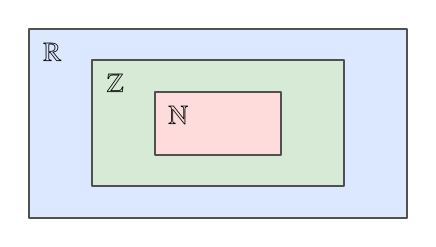
\begin{tikzpicture}[x=1cm,y=1cm, line cap=round, line join=round]

\draw[draw=darkgray, fill=lightblue, line width=0.8pt] (-2.4,-1.2) rectangle (2.4,1.2);
\draw[draw=darkgray, fill=lightgreen, line width=0.8pt] (-1.6,-0.8) rectangle (1.6,0.8);
\draw[draw=darkgray, fill=lightred, line width=0.8pt] (-0.8,-0.4) rectangle (0.8,0.4);

\node at (-2.1,0.9) {$\mathbb{R}$};
\node at (-1.3,0.5) {$\mathbb{Z}$};
\node at (-0.5,0.1) {$\mathbb{N}$};

\end{tikzpicture}
\end{document}
